documentclass[12pt]{article}
\usepackage{tikz}
\usetikzlibrary{calc}
\begin{document}

\begin{figure}[h]
    \centering
    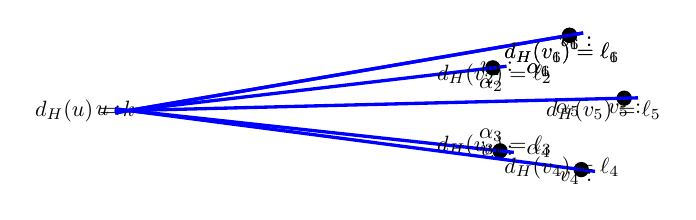
\begin{tikzpicture}[scale=0.9]
    \tikzstyle{myarrow} = [black,-latex,thick];
    \draw (-5,0) node[left,scale=0.8]{$u:$} -- (-4.8,0);
    \draw (-4.8,0) node[left,scale=0.8]{$d_H(u)=k$};
    \foreach \i in {1,...,6}{
        \pgfmathsetmacro{\angle}{36*\i}
        \draw[fill] (\angle+5:{2*cos(\angle)}) circle (0.1cm);
        \draw[blue,very thick,shorten >=-5pt,shorten <=-5pt] (-5,0)--({\angle+5}:{2*cos(\angle)});
        \node[scale=0.8] at ({\angle}:{2*cos(\angle)}) {$v_\i:$};
        \node[scale=0.8] at ({\angle}:{1.7*cos(\angle)}) {$d_H(v_\i)=\ell_\i$};
        \node[scale=0.8] at ({\angle}:{1.2*cos(\angle)}) {$\alpha_\i$};
    }
    \end{tikzpicture}
\end{figure}

\end{document}